% Options for packages loaded elsewhere
\PassOptionsToPackage{unicode}{hyperref}
\PassOptionsToPackage{hyphens}{url}
\documentclass[
]{article}
\usepackage{xcolor}
\usepackage{amsmath,amssymb}
\setcounter{secnumdepth}{-\maxdimen} % remove section numbering
\usepackage{iftex}
\ifPDFTeX
  \usepackage[T1]{fontenc}
  \usepackage[utf8]{inputenc}
  \usepackage{textcomp} % provide euro and other symbols
\else % if luatex or xetex
  \usepackage{unicode-math} % this also loads fontspec
  \defaultfontfeatures{Scale=MatchLowercase}
  \defaultfontfeatures[\rmfamily]{Ligatures=TeX,Scale=1}
\fi
\usepackage{lmodern}
\ifPDFTeX\else
  % xetex/luatex font selection
\fi
% Use upquote if available, for straight quotes in verbatim environments
\IfFileExists{upquote.sty}{\usepackage{upquote}}{}
\IfFileExists{microtype.sty}{% use microtype if available
  \usepackage[]{microtype}
  \UseMicrotypeSet[protrusion]{basicmath} % disable protrusion for tt fonts
}{}
\makeatletter
\@ifundefined{KOMAClassName}{% if non-KOMA class
  \IfFileExists{parskip.sty}{%
    \usepackage{parskip}
  }{% else
    \setlength{\parindent}{0pt}
    \setlength{\parskip}{6pt plus 2pt minus 1pt}}
}{% if KOMA class
  \KOMAoptions{parskip=half}}
\makeatother
\usepackage{longtable,booktabs,array}
\newcounter{none} % for unnumbered tables
\usepackage{calc} % for calculating minipage widths
% Correct order of tables after \paragraph or \subparagraph
\usepackage{etoolbox}
\makeatletter
\patchcmd\longtable{\par}{\if@noskipsec\mbox{}\fi\par}{}{}
\makeatother
% Allow footnotes in longtable head/foot
\IfFileExists{footnotehyper.sty}{\usepackage{footnotehyper}}{\usepackage{footnote}}
\makesavenoteenv{longtable}
\usepackage{graphicx}
\makeatletter
\newsavebox\pandoc@box
\newcommand*\pandocbounded[1]{% scales image to fit in text height/width
  \sbox\pandoc@box{#1}%
  \Gscale@div\@tempa{\textheight}{\dimexpr\ht\pandoc@box+\dp\pandoc@box\relax}%
  \Gscale@div\@tempb{\linewidth}{\wd\pandoc@box}%
  \ifdim\@tempb\p@<\@tempa\p@\let\@tempa\@tempb\fi% select the smaller of both
  \ifdim\@tempa\p@<\p@\scalebox{\@tempa}{\usebox\pandoc@box}%
  \else\usebox{\pandoc@box}%
  \fi%
}
% Set default figure placement to htbp
\def\fps@figure{htbp}
\makeatother
\setlength{\emergencystretch}{3em} % prevent overfull lines
\providecommand{\tightlist}{%
  \setlength{\itemsep}{0pt}\setlength{\parskip}{0pt}}
\usepackage{bookmark}
\IfFileExists{xurl.sty}{\usepackage{xurl}}{} % add URL line breaks if available
\urlstyle{same}
\hypersetup{
  pdftitle={Two Walls{,} Two Rulers: What Context Compaction Actually Drops in a Real Agent Deployment},
  pdfauthor={Anan Long},
  hidelinks,
  pdfcreator={LaTeX via pandoc}}

\title{Two Walls, Two Rulers: What Context Compaction Actually Drops in
a Real Agent Deployment}
\author{Anan Long}
\date{2026-09-22}

\begin{document}
\maketitle

\section{Abstract}\label{abstract}

Long-horizon agents depend on context compaction. Prior work
characterizes compaction using benchmarks, controller-generated
trajectories, and --- in at least one case --- material drawn from real
agent configurations and prompts. We report measurements from a
\textbf{real, continuously used single-machine agent deployment}:
\textbf{48 session directories with at least one successful compaction,
203 successful compactions, and 41 recorded failure attempts} (snapshot
2026-09-19 00:3x local; the deployment keeps running, so every
corpus-level number is paired with its snapshot). We report four
findings, each with a measurement device that runs on ordinary session
logs.

\textbf{(1) Failures are three mechanisms, not one.} Truncation (24),
\emph{no-shrink} (the summary is not smaller than what it shadows; 15),
and a token-meter mismatch (2). Truncation and no-shrink require
\textbf{opposite} remedies: one needs an output-budget strategy, the
other needs a criterion for \emph{refusing to compact} that span. Prior
work measured an output floor; it did not name the failure mode that
occurs below it.

\textbf{(2) Summaries do not carry freshness --- structurally, not by
accident.} The \texttt{Next\ Step} section is written \emph{by the
summarizer, at generation time}, and is rewritten only by the next
compaction: between those two moments it reports as current a state the
session has already moved past. \textbf{The section is not failing at
its job; the job is undefined} --- nothing in the summary format carries
a timestamp or a validity condition. We show the consequence twice, and
the second is the half that carries. \textbf{(a) It is acted on.} In the
behavioural runs (§5), probes given one real summary \textbf{moved on a
waiting condition the live session had already resolved} instead of
reporting it, so the failure does not depend on how the question was
phrased. \textbf{(b) Its form travels with it} --- the half we file as
\textbf{weak}: sixteen zero-history probes retrieved that same resolved
sentence (\textbf{16/16}), a reading that proves little \textbf{by
construction}, because the material states a waiting condition and the
question asks what it waits on, so a faithful reader answers correctly;
we keep it only as the entry point to (a). What it still shows is narrow
and worth one clause: a resolved statement travels in the \textbf{same
surface form, with the same confidence, as a live one} --- because
\textbf{compaction rewrites; it does not timestamp}. (Summary text is
paraphrased rather than quoted: not published, under our own data
policy.)

\textbf{(3) Two rulers, one phenomenon.} Constraint items (the summary's
\texttt{\#\#\ Boundaries} section) survive \textbf{verbatim} at
\textbf{13\%} after one compaction round and \textbf{0\%} by round four.
Judged \textbf{semantically} (three states: verbatim /
reworded-but-present / gone) by ten zero-history judges, the same items
survive at \textbf{91\%}, \textbf{77\%}, and \textbf{53\%} (k = 1, 2,
4). One number per point invites the wrong question, so rounds 2 and 4
were re-judged by \textbf{two further independent sets of readers} (same
packs, same rule, \textbf{102 cells each}). The result splits: the
\textbf{shape reproduces, the deepest point does not} --- k = 2 reads
\textbf{76.8 / 76.8 / 78.6\%}, k = 4 reads \textbf{53.3 / 45.7 / 45.7\%}
(majority \textbf{47.8\%}), while at k = 1 four further readers of the
same 56 cells span \textbf{82.1--91.1\%}. §4 carries each reading, the
interval on every point, and where the movement comes from ---
\textbf{pass-versus-readers, not reader noise}. Reporting \textbf{either
ruler alone inverts the conclusion}, and no single number should be read
as \emph{the} survival rate.

\textbf{(4) Substitution, not fabrication.} In a task-completion
setting, \textbf{twelve probes given the material without a retrieval
card failed to select the operative ``do not touch'' constraint (12/12,
three batches of four) and none of them marked the choice as a guess};
four probes given the same material \textbf{with} a card selected it
(4/4). The card-versus-no-card contrast in the first batch is
significant at this sample size (Fisher exact, two-sided, \textbf{p =
0.029}), and that significance \textbf{rests entirely on the zero}: had
a single no-card probe selected the operative constraint, the two-sided
p would rise to \textbf{0.14} and stop being significant (0.43 at 2/4,
1.00 at 3/4; \texttt{node\ tools/fisher.mjs}). They did not fabricate
--- they substituted a \emph{different} constraint that genuinely
appears in the material. \textbf{The two further batches of four no-card
probes are reported separately rather than pooled}: in the second batch
the frozen task text still pointed the windows at the apparatus document
that records this probe's answer (a defect we found afterwards and
fixed), and in the third batch --- with that pointer removed and the
material moved out of the apparatus tree --- the substituted targets
\textbf{diversified} (two probes took the standing constraint that
appears verbatim in the material, one took its own material path, one
took the repository root). Across all three batches (12 no-card probes,
0 correct) the \emph{zero} replicates: the operative constraint is never
recovered. \textbf{Which} constraint gets substituted does not
replicate, so we do not present ``nearest-hand substitution'' as the
mechanism --- \textbf{the invariant is the miss, not the substitute}.
Across the first eight probes the number of searches was \textbf{0}; the
four probes of the third batch were likewise \textbf{0/4} searches
(scanned from their own session logs).

\textbf{A human pass exists}: one author, blind to the key, agrees with
it more closely than either machine pass (three-state \textbf{56.5\%},
two-state \textbf{89.1\%}) --- our own prediction that human--machine
agreement would be lower is not supported. \textbf{Three further
readers, one from each of three different model families}, judged the
same cells blind; where they differ from one another they split
two-to-one and \textbf{never three ways}, and every disagreement with
the key sits on the wording seam --- \textbf{never} on whether a
constraint survived. We do not claim a fix. Prior work shows that
re-surfacing a plan does not restore task success; our positive results
cover \textbf{state understanding}, not \textbf{behavioral success}.

\begin{center}\rule{0.5\linewidth}{0.5pt}\end{center}

\section{Introduction}\label{introduction}

Long-horizon agents survive their own context window by compacting: an
LLM summarizes the older part of a conversation, the summary replaces
what it shadowed, and work continues. Every deployed system does some
version of this, and the measurements that exist are mostly on
benchmarks and controller-generated trajectories. This paper measures
\textbf{one deployment that has been in continuous use} --- a
single-machine agent whose session logs record every compaction it has
performed --- and asks a narrower question than ``does compaction
help'': \textbf{what does it actually drop, and can the system tell?}
\textbf{Material and method.} 48 session directories, 203 successful
compactions and 41 recorded failure attempts at the §1.2 snapshot. The
corpus is \textbf{live}, so every corpus-level number is quoted with the
snapshot it was taken at; devices run on ordinary session logs, with no
instrumentation of the compactor, and each is given an input whose
answer we already knew: a fixpoint that must be 100\%, a synthetic
foreign corpus, and a positive control that must fail when the
assumption behind it is wrong. \textbf{Contributions.} - \textbf{C1
(load-bearing).} Failures are \textbf{three} mechanisms, not one ---
truncation (24), \emph{no-shrink} (15) and a token-meter mismatch (2)
--- and the first two need \textbf{opposite} remedies. Extended on the
success side: the meter and the failure signal \textbf{disagree on about
9\%} of successful compactions (20 of 231 --- the live library on
2026-09-20, a different moment from the §1.2 snapshot; §2). - \textbf{C2
(a single structural observation).} A summary carries \textbf{no
freshness}: the \texttt{Next\ Step} section is written at generation
time and rewritten only by the next compaction, so an already-resolved
state travels as current, and the section is not failing at its job ---
the job is undefined (§3). - \textbf{C3 (load-bearing).} Constraint
survival depends entirely on the ruler: \textbf{13\% → 5\% → 0\%}
verbatim (normalized 5-gram) but \textbf{91 / 77 / 53\%} semantically
across independent zero-history judges --- and the least stable of those
points is the one we headline (§4). - \textbf{C4 (a direction, not a
rate).} Given the material \textbf{without} a retrieval card, \textbf{12
of 12} probes failed to retrieve the operative constraint and none
marked uncertainty; with a card, 4 of 4 did. \textbf{The miss
replicates; the substitute does not} (§5). \textbf{What we do not do.}
We claim \textbf{no fix}. Prior work shows that re-surfacing a plan does
not restore task success, and our own material shows the same shape; we
report what we measured, where we measured it, and what would falsify it
(§7, §8).

\textbf{What we would try next, in order.} (i) \textbf{Refuse to
compact} a span whose summary is not smaller than what it shadows ---
the criterion \emph{no-shrink} names, and the one place where nothing in
the current design tells the operator to stop. (ii) \textbf{Carry
validity on generated sections}: a \texttt{Next\ Step} that records when
it was written and what would invalidate it, so a resolved state cannot
present itself as current. (iii) \textbf{Make the retrieval card
mandatory at task start} rather than optional --- the arm C4 measures.
We claim \textbf{no effect} for any of the three. Each is a direction
our own readings point at, and each is falsifiable with the devices used
in §2--§5.

\textbf{What is about the step, and what is about this machine.} The
failure taxonomy and the timestampless section are statements about the
compaction step \textbf{as specified here} --- a compactor with an
output budget, a size check, and no validity field --- and any
deployment whose logs record the same events can re-run the devices that
produce them. Every \emph{rate} we report is a rate about \textbf{one}
deployment at a \textbf{named snapshot}, and each is quoted with its
snapshot where it appears.

\section{1. Setting and corpus}\label{setting-and-corpus}

\subsection{1.1 The deployment}\label{the-deployment}

The setting is a single-machine agent harness used continuously by one
person for work, study, and personal assistance. Sessions are persisted
as append-only logs, one directory per session. Agent turns, tool calls,
and context events are recorded as typed events; context management
(compaction) is a plug-in component of the harness, not a wrapper around
it.

A \textbf{generation} is one successful compaction: a span of the
session's message history is replaced by a generated summary. The
harness emits, per generation:

\begin{itemize}
\tightlist
\item
  a \texttt{compaction/summary} event carrying the summary text;
\item
  a \texttt{compaction/receipt} event carrying a \textbf{deterministic
  retention audit}: which declared sections are missing from the summary
  prose, and which file paths and \texttt{UPPER\_SNAKE} identifiers
  present in the shadowed original (or in the verbatim spill) are absent
  from it. \textbf{The receipt carries no token field} --- the shadowed
  span's estimate (\texttt{shadowedTokenCount}) is on
  \texttt{compaction/summary}, and the summary side has only the
  summarization call's own usage, so the two numbers sit on
  \textbf{different metering channels} (§2, token-meter); (F1 receipt)
\item
  the identity of the spans that were shadowed, including, in most
  generations, the \emph{previous summary} itself.
\end{itemize}

A \textbf{failure attempt} is a \texttt{compaction/failure}-class event
carrying the harness's own error string. We count attempts, not
sessions, and deduplicate where the same conversation was recorded under
more than one directory.

\subsection{1.2 Scale}\label{scale}

{\def\LTcaptype{none} % do not increment counter
\begin{longtable}[]{@{}
  >{\raggedright\arraybackslash}p{(\linewidth - 2\tabcolsep) * \real{0.5000}}
  >{\raggedright\arraybackslash}p{(\linewidth - 2\tabcolsep) * \real{0.5000}}@{}}
\toprule\noalign{}
\begin{minipage}[b]{\linewidth}\raggedright
Quantity
\end{minipage} & \begin{minipage}[b]{\linewidth}\raggedright
Value (snapshot 2026-09-19 00:3x)
\end{minipage} \\
\midrule\noalign{}
\endhead
\bottomrule\noalign{}
\endlastfoot
Session directories with \ensuremath{\geq}1 successful compaction &
\textbf{48} \\
Successful compactions & \textbf{203} \\
Recorded failure attempts & \textbf{41} (in 6 sessions; de-duplicated
lower bound 37) \\
Generations per session & median \textbf{2}, mean \textbf{4.2} ---
heavy-tailed \\
Concentration & two 29-generation sessions (\ensuremath{\approx}4\% of
sessions) hold 58 of 203 generations (\ensuremath{\approx}29\%) \\
\end{longtable}
}

\textbf{The corpus is alive, and that is a methodological hazard.} The
same measurement pipeline four hours earlier (2026-09-18 17:2x) reported
46 / 192 / 41. A reader who recomputes and disagrees should check the
snapshot before the method.

The deepest single session ran 29 generations across ten days: 29
summaries totalling 359,853 characters, of which \textbf{99.4\% is text
carried over from the summary that was itself consumed} --- the
compaction chain is a relay, not a funnel.

\emph{Evidence:}
\texttt{tools/compaction-census.mjs\ list\textbar{}show\textbar{}chain};
per-session aggregate columns in \texttt{data/sessions.md} (anonymized
\texttt{S01..S48}; the identity mapping is not published).

\subsection{1.3 Method}\label{method}

All four findings come from one pipeline: decode session logs → extract
compaction events and their receipts → derive per-generation tables →
apply a fixed criterion (written into the device header before use). The
criterion is stated where it is applied, never in this text alone:
changing a threshold means changing the device.

\textbf{Use of AI tools.} Reported under arXiv's policy on generative AI
language tools. An agent inside the deployment under study (\texttt{D},
a text-to-text generative tool) wrote the measurement devices, ran them,
and drafted this report. The human author set the questions, reviewed
each device against its inputs, checked every reported number against
the device output, and \textbf{takes full responsibility for all
contents, irrespective of how any part was generated}. Two consequences
are recorded rather than left implicit: (i) the annotation key and the
judges of §4/§8 come from \textbf{the same system under study} (§8, item
2); (ii) every work cited in §6 was checked against its own arXiv or
publisher page (title, year, venue where one exists), and quoted
sentences were matched against the source text --- unchecked references
are what the policy targets.

\section{2. Finding 1 --- failures are three
mechanisms}\label{finding-1-failures-are-three-mechanisms}

\pandocbounded{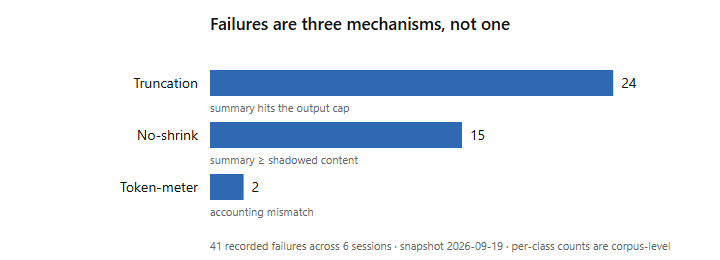
\includegraphics[keepaspectratio]{fig1-failures.png}}

\textbf{Figure 1.} Failure mechanisms recorded in this deployment (n =
41 attempts): truncation 24, no-shrink 15, token-meter 2.

{\def\LTcaptype{none} % do not increment counter
\begin{longtable}[]{@{}
  >{\raggedright\arraybackslash}p{(\linewidth - 6\tabcolsep) * \real{0.2500}}
  >{\raggedright\arraybackslash}p{(\linewidth - 6\tabcolsep) * \real{0.2500}}
  >{\raggedright\arraybackslash}p{(\linewidth - 6\tabcolsep) * \real{0.2500}}
  >{\raggedright\arraybackslash}p{(\linewidth - 6\tabcolsep) * \real{0.2500}}@{}}
\toprule\noalign{}
\begin{minipage}[b]{\linewidth}\raggedright
Mechanism
\end{minipage} & \begin{minipage}[b]{\linewidth}\raggedright
Verbatim error text
\end{minipage} & \begin{minipage}[b]{\linewidth}\raggedright
Count
\end{minipage} & \begin{minipage}[b]{\linewidth}\raggedright
Remedy direction
\end{minipage} \\
\midrule\noalign{}
\endhead
\bottomrule\noalign{}
\endlastfoot
Truncation &
\texttt{summarization\ truncated\ at\ the\ token\ cap\ (incomplete\ checkpoint)}
& 24 & raise or segment the output budget \\
\textbf{No-shrink} &
\texttt{summary\ is\ not\ smaller\ than\ the\ shadowed\ content\ (4389\ estimated\ framed\ tokens\ \textgreater{}=\ 3952)}
& 15 & a criterion for \textbf{not} compacting this span \\
Token-meter & (accounting mismatch on a different channel of the same
session) & 2 & fix the measurement, not the compactor \\
\end{longtable}
}

The two dominant mechanisms are not variations of one disease.
Truncation is an output-capacity failure --- the summary was never
finished. No-shrink is the opposite: the summary \emph{was} finished and
is not smaller than what it replaced, so compaction spent budget to save
none. In the recorded case above, the framed summary exceeds the
shadowed span by \textbf{437 estimated tokens}: the operation strictly
increased context cost.

No-shrink is possible precisely because summarizers bound their own
output. The literature has measured that floor (``output volume is
essentially input- and prompt-invariant across four backbones spanning
8B to 120B parameters''). What has not been named is the failure that
occurs when the floor meets a span that is already small: the operator
should stop, and nothing in the current design tells it to. In our
corpus the two mechanisms co-occur in the same deployment and sometimes
in the same session, which is why we report them as separate classes
rather than as one failure rate.

\textbf{Why this is not the intuitive failure.} A successful compaction
is recorded as a success: the summary replaces the span, the session
continues, and nothing downstream compares the two. Where the two
records disagree --- the summarizer's own metering beside the shadowed
estimate (later in this section) --- they are read by different
consumers at different times, and neither is a gate. No-shrink is quiet
for the opposite reason: the harness refuses, the session goes on, and
the cost is visible only to a reader who counts
\texttt{compaction/failure} events rather than
\texttt{compaction/summary} ones.

\subsection{Alternative explanations we could not rule
out}\label{alternative-explanations-we-could-not-rule-out}

\begin{itemize}
\tightlist
\item
  \textbf{The token estimate may be the artifact.} No-shrink is decided
  from the harness's \emph{estimated framed tokens}, not from measured
  usage. If that estimate is biased for short spans, some no-shrink
  events may be measurement artifacts rather than genuine
  non-reductions. We see no way to check it without instrumenting the
  compactor, which we did not do.
\item
  \textbf{Attempts vs.~outcomes.} We count failure \emph{attempts}. We
  do not know how often an attempt was retried successfully, so 41 is
  not ``41 losses''; it is 41 recorded refusals or errors.
\item
  \textbf{Class boundary.} The third class (token-meter, n=2) was
  identified on a single session and may be an instance of the first two
  seen through a different channel.
\end{itemize}

\begin{quote}
\textbf{Threat note.} An output floor is known; the \emph{no-shrink}
failure mode below it is, to our knowledge, unnamed. \textbf{Failure
signals catch only the extreme; on a second channel, one success in
twelve is not smaller.} The \texttt{no-shrink} decision above is made on
the harness's own \emph{estimated framed tokens}. The summarization call
records, on the same event, its own metering next to the span it
replaced (\texttt{usage.outputTokens} beside
\texttt{shadowedTokenCount}). Over \textbf{231 successful compactions
with both fields present} (live library, 2026-09-20 --- a different
moment from the §1.2 snapshot; zero missing values), \textbf{20 (8.7\%)
report provider output tokens at or above the shadowed estimate}.
\textbf{All 20 sit in one of the four workspaces} in the library (122
successes there; 100 + 6 + 3 in the other three combined, none
net-negative) and their spans are small (1.1k--2.6k estimated tokens;
library median ratio 0.034). Two different readers are piled into that
sentence and must be separated: provider \texttt{outputTokens} measures
\textbf{what the model generated}, not what was retained --- for the
worst cases a third ruler on the retained summary text (characters ÷ 4)
puts it at \ensuremath{\approx}0.7--0.9 of the shadowed span while the
provider reports 1.5--2.2×. So the defensible claim is narrower than
``the operation was net-negative'': \textbf{the record of extreme
failures and the record of metering disagree on about 9\% of successful
compactions}, which is the token-meter family of §2's third class seen
at scale rather than at n = 2. Positive control: the 15 recorded
no-shrink refusals parse to \emph{A \ensuremath{\geq} B} in all 15
(median A/B = 1.000) --- where the harness itself refused, the two
channels agree. Reproduce with \texttt{node\ tools/net-shrink.mjs} (it
prints its own control and refuses to run if the control fails).
\end{quote}

\section{3. Finding 2 --- summaries do not carry
freshness}\label{finding-2-summaries-do-not-carry-freshness}

Sixteen zero-history probes were given a single input: a real summary
produced by this deployment's compactor. Among the summary's sections is
\texttt{Next\ Step}, which at generation time recorded that the session
was \textbf{waiting for the user to decide} a design question --- a
decision the live session had already made by the time the probes read
the summary.

\textbf{16 of 16 probes retrieved that sentence} and reported it as the
current blocking condition. In the live session, that decision had
already been made and carried out --- the very compaction under study
was its execution. The summary was correct about the past and wrong
about the present, and the probes had no instrument to tell the
difference, because \textbf{compaction rewrites; it does not timestamp}.

A structural instance of the same problem: the \texttt{Next\ Step}
section is written by the summarizer at generation time, so it is stale
from the moment it is written until the next compaction rewrites it. The
section is not failing at its job; the job is undefined.

\subsection{Alternative explanations we could not rule
out}\label{alternative-explanations-we-could-not-rule-out-1}

\begin{itemize}
\tightlist
\item
  \textbf{Question priming.} The probes were asked what the material
  says is being waited on. A question phrased differently might elicit a
  hedged answer. (In the behavioural runs, §5, the same pattern appears
  without any such question: probes acted on the stale state rather than
  reporting it.)
\item
  \textbf{One material family.} All sixteen probes read summaries from
  the same deployment and the same generation lineage. We have not shown
  that freshness loss is \emph{general}; we have shown that at least one
  real, load-bearing statement came back dead, sixteen times out of
  sixteen.
\item
  \textbf{No timestamp field.} The comparison is not ``the summary
  forgot a timestamp''; the harness does not put one there. Whether
  adding one would help is untested.
\end{itemize}

\begin{quote}
\textbf{Threat note.} Related work measures \emph{content loss} (rules
erased, plans evicted, fidelity decay). Freshness is a different axis:
an item can be perfectly preserved and simultaneously expired.
\end{quote}

\section{4. Finding 3 --- two rulers, one
phenomenon}\label{finding-3-two-rulers-one-phenomenon}

\pandocbounded{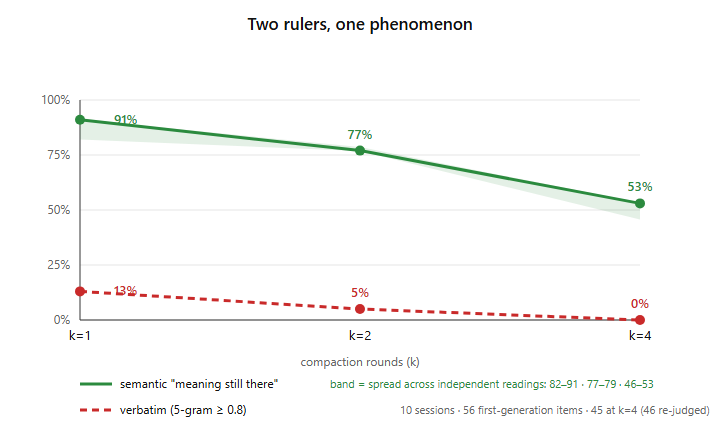
\includegraphics[keepaspectratio]{fig2-two-rulers.png}}

\textbf{Figure 2.} Two rulers on the same materials: verbatim survival
13 / 5 / 0\% and semantic survival 91 / 77 / 53\% at k = 1, 2, 4; the
band is the spread across independent judges.

We measured constraint survival two ways \textbf{on the same materials},
across 10 sessions whose summaries contain a \texttt{\#\#\ Boundaries}
section --- the section the harness's own summarizer instruction
declares as \emph{constraints and out-of-scope: what NOT to do}
(\texttt{compaction-basic/src/sections.ts:33}), i.e.~the deployment's
own name for its constraint section (\textbf{56} first-generation items;
\textbf{46} in the k = 4 pool of the current device, \textbf{45} in the
earlier extraction --- see the note under the table):

{\def\LTcaptype{none} % do not increment counter
\begin{longtable}[]{@{}
  >{\raggedright\arraybackslash}p{(\linewidth - 4\tabcolsep) * \real{0.3333}}
  >{\raggedright\arraybackslash}p{(\linewidth - 4\tabcolsep) * \real{0.3333}}
  >{\raggedright\arraybackslash}p{(\linewidth - 4\tabcolsep) * \real{0.3333}}@{}}
\toprule\noalign{}
\begin{minipage}[b]{\linewidth}\raggedright
k (compaction rounds)
\end{minipage} & \begin{minipage}[b]{\linewidth}\raggedright
verbatim (normalized, 5-gram \ensuremath{\geq} 0.8)
\end{minipage} & \begin{minipage}[b]{\linewidth}\raggedright
semantic (``meaning still there'')
\end{minipage} \\
\midrule\noalign{}
\endhead
\bottomrule\noalign{}
\endlastfoot
1 & \textbf{13\%} (7/56 · 95\% CI 6--24\%) & \textbf{91\%} (51/56 · 95\%
CI 81--96\%) \\
2 & 5\% & 77\% \\
4 & \textbf{0\%} (0/46)* & \textbf{53\%} (24/45)† \\
\end{longtable}
}

\emph{* verbatim pool (46 bullets) · † pass-1 semantic cells (45) ---
the note below says why the two bases differ. Intervals are
\textbf{Wilson 95\% score intervals}, given where the counts are stated
(k = 1); at k = 2 and k = 4 the dominant uncertainty is \textbf{reader
spread}, reported in the next subsection.}

\textbf{Two denominators at k = 4 --- and the difference is one
\emph{judged cell}, not one item.} The verbatim ruler's pool holds
\textbf{46} bullets: the hand-sum of the generation-1 counts over the
eight sessions that reach k = 4 (\textbf{7+5+9+5+6+4+5+5}, printed per
session by \texttt{tools/constraint-survival.mjs}). The semantic reading
tallies \textbf{45} cells at k = 4 in pass 1 and \textbf{46} after
re-judging, and the single extra cell is visible in the tally device's
own output: in pass 1 that cell came back \textbf{\texttt{unjudgeable}
--- an answer outside the three-state vocabulary} (its later summary had
kept only a place name for an item of personal information), so it was
excluded from the pass-1 counts, and the re-judging pass answered it
inside the vocabulary. The figure's footer names both bases (``45 at k =
4 (46 re-judged)''). \textbf{Both bases give the same verbatim zero},
and the excluded cell is \textbf{not counted as a survival in either
pass}. §8's agreement figures (\textbf{52.2\%}, \ensuremath{\kappa} =
0.226) are a \textbf{different quantity on a different base} ---
agreement with the key --- not a second estimate of the survival rate.

The semantic column comes from ten zero-history judges, each reading one
self-contained pack: the generation-1 constraint list, then the later
summary. Each judge answered a three-state question --- \emph{verbatim}
/ \emph{reworded but present} / \emph{gone} --- with a quoted basis,
under an explicit ``if you cannot find it, say \texttt{gone}'' rule. The
pack contained nothing else: no question about the study, no hint about
the hypothesis.

Four conclusions:

\begin{enumerate}
\def\labelenumi{\arabic{enumi}.}
\tightlist
\item
  \textbf{Compaction preserves meaning, not wording.} The gap is
  \ensuremath{\approx}7× at the first round. A study reporting only the
  verbatim ruler would conclude that constraints are destroyed; a study
  reporting only the semantic ruler would conclude compaction is safe.
  Both would be reporting the same experiment.
\item
  \textbf{The two decay at different rates} (semantic: 91 → 77 → 53,
  each point carrying an interval; verbatim: 13 → 5 → 4 → 0). ``Verbatim
  death'' is therefore not evidence of ``constraint death'' --- and,
  conversely, a carrier designed to preserve \emph{wording} addresses a
  different problem (a later window unable to quote the original) than a
  carrier designed to preserve \emph{meaning}.
\item
  \textbf{A structural observation:} the \texttt{\#\#\ Boundaries}
  \emph{section} was never missing across generations (0 of 10 sessions
  lost the heading); what decays is the \textbf{items inside it}. The
  skeleton is stable; contents are rewritten each generation.
\item
  \textbf{Cross-device check.} An independently written device that
  measures strict verbatim inheritance over \emph{all} bullet lines
  reports 4.6\% average inheritance (2,131 distinct lines; only 16 lines
  survive \ensuremath{\geq}3 generations, covering 1.0\% of the final
  generation's characters). A stricter ruler must produce a smaller
  number than a looser one; observed 4.6\% \ensuremath{\leq} 13\%,
  consistent.
\end{enumerate}

\subsection{Stability of the semantic
column}\label{stability-of-the-semantic-column}

One number per point invites the wrong question, so rounds 2 and 4 were
re-judged by \textbf{two further independent sets of readers} (same
packs, same rule, one cell per line, \textbf{102 cells each}): \textbf{k
= 2: 76.8 / 76.8 / 78.6\%} (original · re-read A · re-read B;
\textbf{majority of three 78.6\%}) and \textbf{k = 4: 53.3 / 45.7 /
45.7\%} (\textbf{majority 47.8\%}). The \textbf{shape reproduces and the
deepest point does not} --- k = 2 moves \textbf{1.8} points between
readings, \textbf{k = 4 moves 7.6}, and both fresh readings land below
the original. At k = 1, four further readers of the same 56 cells span
\textbf{82.1--91.1\%} (the \ensuremath{\kappa} reading). Every interval
is drawn in \textbf{Figure 2}. \textbf{Stability is not uniform across
k, and the least stable point is the one we headline}: k = 1 spans
\textbf{9.0 points} across four independent readings (82.1--91.1\%), k =
2 moves \textbf{1.8}, k = 4 moves \textbf{7.6} --- so the deepest point
is \emph{not} the least reliable one, and our \textbf{headline 91\%
carries the widest spread of the three}. That is a result about the
ruler, not an apology about error bars: near ``almost everything is
still there'', independent readers disagree most about which near-misses
count.

\textbf{Where the movement comes from.} The two re-reads agree with each
other on \textbf{87 of 102 cells (85.3\%}; k = 2 80.4\%, k = 4 91.3\%),
and of their 15 disagreements \textbf{10 fall on the boundary the curve
does not use} (\emph{verbatim} \ensuremath{\leftrightarrow}
\emph{reworded}) and \textbf{5 on the one it does} (\emph{still there}
\ensuremath{\leftrightarrow} \emph{gone}). The point itself moves
through a \textbf{different, larger set}: at k = 4 the \textbf{original
pass and the two re-reads} disagree on \textbf{6 cells} (4 where the
original said \texttt{still\ there} and both re-reads said
\texttt{gone}; 2 the reverse; k = 2: 3 cells, net +1)
\ensuremath{\Rightarrow} the shift is \textbf{pass-versus-readers, not
reader noise}. One of those six takes a nameable shape: the later
summary \textbf{generalized the item until its object is no longer
named} (the red line survives as ``do not claim unlanded capability'',
with the \emph{specific} capability --- and the layer distinction ---
gone), so both fresh readers called it \texttt{gone} where the original
called it \texttt{reworded}.

\subsection{Why the judges differ: one seam, not one
disagreement}\label{why-the-judges-differ-one-seam-not-one-disagreement}

Three further readers --- \textbf{three different model families}, same
packs, same rule, blind to the key --- labelled all 56 cells. Where they
disagree with one another they split \textbf{two-to-one and never three
ways} (14 of 56 cells), and \textbf{11 of those 14 sit on the
\texttt{verbatim} \ensuremath{\leftrightarrow} \texttt{reworded} edge};
collapsed to the two states the curve actually uses, the three agree on
\textbf{53 of 56 cells (94.6\%)}.

{\def\LTcaptype{none} % do not increment counter
\begin{longtable}[]{@{}
  >{\raggedright\arraybackslash}p{(\linewidth - 8\tabcolsep) * \real{0.2000}}
  >{\raggedright\arraybackslash}p{(\linewidth - 8\tabcolsep) * \real{0.2000}}
  >{\raggedright\arraybackslash}p{(\linewidth - 8\tabcolsep) * \real{0.2000}}
  >{\raggedright\arraybackslash}p{(\linewidth - 8\tabcolsep) * \real{0.2000}}
  >{\raggedright\arraybackslash}p{(\linewidth - 8\tabcolsep) * \real{0.2000}}@{}}
\toprule\noalign{}
\begin{minipage}[b]{\linewidth}\raggedright
reader (A/B/C = three model families)
\end{minipage} & \begin{minipage}[b]{\linewidth}\raggedright
\texttt{verbatim} \ensuremath{\leftrightarrow} \texttt{reworded}
\end{minipage} & \begin{minipage}[b]{\linewidth}\raggedright
\texttt{reworded} \ensuremath{\leftrightarrow} \texttt{gone}
\end{minipage} & \begin{minipage}[b]{\linewidth}\raggedright
\texttt{verbatim} \ensuremath{\leftrightarrow} \texttt{gone}
\end{minipage} & \begin{minipage}[b]{\linewidth}\raggedright
two-state vs key
\end{minipage} \\
\midrule\noalign{}
\endhead
\bottomrule\noalign{}
\endlastfoot
A & \textbf{14} & 7 & \textbf{0} & 87.5\% \\
B & \textbf{16} & 6 & \textbf{0} & 89.3\% \\
C & \textbf{17} & 6 & \textbf{0} & 89.3\% \\
\end{longtable}
}

That is what the disagreement is: \textbf{not about whether a constraint
survived, but about how much rewording still counts as
\texttt{verbatim}} --- the threshold our own rule never pinned down. The
three ran one pack at a time, in order, inside a single session each, so
unlike the pack-isolated passes their later judgments carry earlier
context; we checked that separately and it points the other way (the
pack-isolated passes lose \textbf{-35.0} and \textbf{-16.5} points
between the first and second half of the material, these three
\textbf{-19.0 / -8.5 / +1.9}), so the residual is not carry-over. They
are reported as \textbf{their own arm} and are \emph{not} folded into
the judge decomposition above, whose counts depend on which judges are
included.

\subsection{A secondary effect we measured and do not
claim}\label{a-secondary-effect-we-measured-and-do-not-claim}

In a separate eight-probe comparison, the \emph{order} of two constraint
bullets in the same material moved selection between them (38\% → 75\%
selecting the operative one when the two lines were swapped). The effect
is directionally consistent across two rounds but \textbf{not
statistically significant} (Fisher exact, two-sided, p = 0.31; a placebo
swap left the other column unchanged, p = 1.0), and we stopped expanding
the sample because the test statistic is non-monotonic in n and ``expand
until p \textless{} 0.05'' is selection, not measurement. We report it
as an observation about \emph{which} constraint a window picks, not
about whether it picks one at all.

\subsection{Alternative explanations we could not rule
out}\label{alternative-explanations-we-could-not-rule-out-2}

\begin{itemize}
\item
  \textbf{The verbatim ruler penalizes paraphrase by construction.} That
  is its purpose; the semantic ruler exists because the verbatim number
  alone is not a statement about loss of meaning.
\item
  \textbf{The judges are ours.} Thresholds, item splitting, and the
  three-state definition were written by the authors, and the judges
  were instantiated by the same system. \textbf{Two machine passes} have
  since been run --- ten zero-history judges each, one pack per judge,
  each forbidden to read any other pack, covering all 56 cells --- the
  second pass on a disambiguated version of the three-state rule,
  because pass 1 left a seam in our own wording (a sentence moved
  word-for-word into another section satisfied both \texttt{verbatim}
  and \texttt{reworded}). \textbf{We measure stability between passes,
  not against the key}: the key is one rater among five and the
  reference the survival curve is built on, not ground truth (§8 states
  the same limit). De-duplicated agreement with it was \textbf{52.2\%
  (Cohen's \ensuremath{\kappa} = 0.226)} in pass 1 and \textbf{54.3\%
  (\ensuremath{\kappa} = 0.261)} in pass 2 --- 25 then 24 disagreements
  out of 56; \textbf{between passes} the figures are \textbf{66--87.5\%
  (three-state)} and \textbf{89--96\% (two-state)} across the four
  independent runs, and those are the numbers we treat as the stability
  of the semantic column. \textbf{Clarifying the rule did not recover
  the disagreement}, so what remains is \textbf{judgment variance, not a
  rule defect}. \textbf{Neither figure is an inter-annotator number in
  the human sense}: same model, no history, and key and passes share a
  model, so a human-versus-model figure can only be lower. Where the
  disagreement sits is still informative: the \texttt{verbatim}
  \ensuremath{\leftrightarrow} \texttt{reworded} boundary carries the
  largest block (18 of 25, then 15 of 24) --- a distinction the survival
  curve never uses. Collapsing to the two states the curve actually uses
  (\emph{still there} vs \emph{gone}) gives \textbf{87.5\% /
  \ensuremath{\kappa} = 0.470} in pass 1 but \textbf{83.9\% /
  \ensuremath{\kappa} = 0.319} in pass 2, so that boundary should be
  quoted as a \textbf{range (83--88\%, \ensuremath{\kappa} 0.32--0.50
  across two runs), not a point} --- with 56 cells we make no
  significance claim between the runs. (Those two-state figures are
  \textbf{per cell}; de-duplicated they are \textbf{87.0\% /
  \ensuremath{\kappa} = 0.502} and \textbf{82.6\% / \ensuremath{\kappa}
  = 0.336}. The three-state numbers earlier in this bullet are
  \textbf{de-duplicated} --- we label each rather than quoting one ruler
  for both.) One further reading is worth stating because it points away
  from the judges: \textbf{the two passes agree with each other on 42 of
  56 cells (75.0\%), while each agrees with our key at 55--57\%}.
\item
  The outlier looked like the \textbf{key} --- which was written while
  reading the whole session, whereas a judge sees only its pack. A
  \textbf{third pass} moves that reading and we now retract it: same
  material, same rule, but judged \textbf{one cell at a time}, so the
  reader never sees a cell's siblings. With three windows the key stands
  alone on only \textbf{10 of 56} cells at three-state resolution and
  \textbf{3 of 56} on the two-state boundary, while the windows disagree
  \emph{among themselves} on \textbf{24} and \textbf{6} cells
  respectively. \textbf{Two windows agreeing is therefore not consensus}
  --- only a third window separates ``agreement'' from ``these two
  happen to match''; with two passes we had been reading the former as
  the latter. The third pass also sits \textbf{closer to the key}
  (92.9\% two-state) than either pack-level pass (87.5\%, 83.9\%), which
  is consistent with the key having been written item by item rather
  than pack by pack --- but the contrast is \textbf{not significant}
  (McNemar exact, p = 0.238 / 0.302 three-state; 0.375 / 0.063
  two-state), so we report a direction, not a result.
\item
  A \textbf{fourth pass} closes the loop on the ``our judges are the
  problem'' worry: a \textbf{different vendor's model} (Claude), given
  the same packs and the same rule, agrees with our key on
  \textbf{64.3\%} of cells --- 89.3\% on the two-state boundary --- and
  lands inside the same band as the machine passes. With four judges the
  key stands alone on only \textbf{2 of 56} boundary cells while the
  judges disagree among themselves on 8; \textbf{no pass is a systematic
  outlier} at any judge count, and the ordering that would say position
  matters more than model family (cell-level and cross-model raters
  agree with each other on 87.5\% of cells, the highest pair in the
  matrix) is \textbf{not significant} (McNemar exact, p
  \ensuremath{\geq} 0.267). We report it as a hypothesis for a dedicated
  run, not as a result. A same-pack control (one pack judged twice by
  two independent zero-history windows under the identical clarified
  rule) came out \textbf{5 of 7 cells}.
\item
  A \textbf{four-judge decomposition} (key / pass 1 / pass 2 / pass 3 /
  cross-model pass, per cell) puts numbers on it --- \textbf{Figure 3}
  draws these same 56 cells, aggregate counts only --- and the numbers
  moved as judges were added: on the three-state labels all four judges
  agree with the key on \textbf{39.3\%} of cells, all four agree with
  each other but differ from the key on \textbf{16.1\%}, and the judges
  disagree \emph{among themselves} on \textbf{44.6\%} --- the largest
  block. On the two states the curve actually uses, the same
  decomposition is \textbf{82.1\% / 3.6\% / 14.3\%}: there the key
  stands alone on only \textbf{two} cells while the judges disagree with
  each other on \textbf{eight}. (Judge counts are not comparable to one
  another --- more judges make consensus harder --- so we read this as
  ``no systematic outlier at any count'', not as a trend.) \textbf{With
  two passes we had read ``the two agree'' as consensus and called the
  key the outlier; neither the third judge nor the cross-model judge
  supports that reading} --- which is why the sentence above is stated
  as a retraction. We then tested the most convenient explanation for
  that --- that our key simply applied an older reading of the rule (the
  disambiguation was written \emph{after} the key) --- and it fails:
  among the 16 cells where our key stood alone against the first two
  passes, only \textbf{3 (19\%)} have the original wording still present
  verbatim in the later summary, against \textbf{7 of 25 (28\%)} among
  the agreed cells (criterion: normalized 5-gram containment
  \ensuremath{\geq} 0.8, a verbatim proxy, not a semantic test). The
  divergence is substantive, not an artefact of rule version. By that
  same proxy, \textbf{3 of those 16} cells have the wording still
  present, yet our key says \texttt{reworded} --- and under a stricter
  criterion (the item's full normalized text as a contiguous substring
  of the later summary) it is \textbf{1 of those 16}. Both counts are
  recorded as instrument defects in the key, not as properties of the
  corpus; the two criteria are monotone here (strict
  \ensuremath{\subseteq} proxy, 3 of 56 vs 17 of 56, no reversals). Both
  figures are reported with the instrument defects attached, not as a
  property of the corpus, and the semantic column should still be read
  as a first measurement with wide error bars rather than a rate.
\item
  \textbf{A human pass now exists, and it narrows that bar rather than
  widening it.} One of the authors --- the human half of the
  deployment's pair; the key and both machine passes were produced by
  the agent half --- labelled all 56 cells after reading only the packs
  and the three-state rule, with no access to the key. Three-state
  agreement with the key is \textbf{57.1\% per cell / 56.5\%
  de-duplicated (\ensuremath{\kappa} = 0.282 / 0.291)}, i.e.~\textbf{at
  or above both machine passes}, so the machine figures are not an upper
  bound on human agreement: the prediction in our previous draft (``a
  human-versus-model figure can only be lower'') is \textbf{falsified},
  and we record the retraction rather than the prediction. Her
  disagreements concentrate where the machine passes' did: \textbf{19 of
  24 sit on the \texttt{verbatim} \ensuremath{\leftrightarrow}
  \texttt{reworded} edge} (machine passes: 18 of 25, then 15 of 24),
  against 5 on \texttt{reworded} \ensuremath{\leftrightarrow}
  \texttt{gone}. On that edge she leans in \textbf{both} directions ---
  10 cells toward \texttt{reworded} where the key said
  \texttt{verbatim}, 9 the other way --- where each machine pass leans
  one way (11 and 10 cells toward \texttt{verbatim}). On the two states
  the survival curve actually uses she is \textbf{the closest of the
  three raters to the key: 91.1\% per cell / 89.1\% de-duplicated
  (\ensuremath{\kappa} = 0.568 / 0.556)}, leaving \textbf{5 of 56} cells
  in dispute (machine passes: 7 and 9). Her pass ran under the
  \textbf{original} three-state rule --- the packs' own version, the one
  this bullet opens with a seam in --- not the disambiguated rule. With
  \textbf{three raters, one of them an author}, this is still not a
  general inter-annotator study; it is the human tier this report was
  missing.
\end{itemize}

\pandocbounded{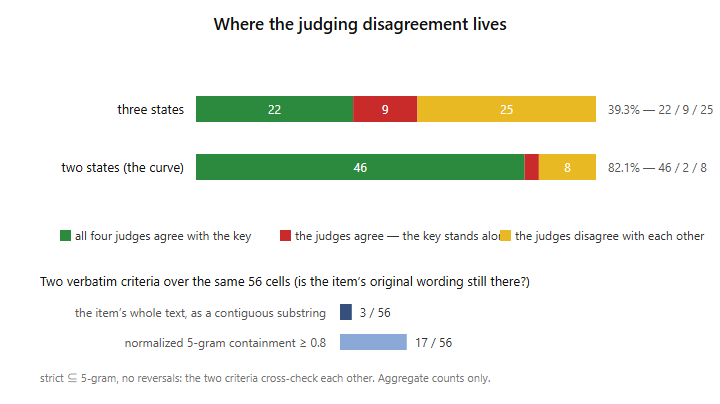
\includegraphics[keepaspectratio]{fig3-judging-decomposition.png}}

\textbf{Figure 3.} Where judging disagreement sits across 56 cells:
39.3\% --- 22 / 9 / 25 on the three-state labels, and 82.1\% --- 46 / 2
/ 8 on the two states the curve uses.

\begin{itemize}
\tightlist
\item
  \textbf{Item granularity.} A compound constraint (``full authority,
  but report back'') can have one half present and one half gone; the
  three-state scheme collapses that to one label. One judge reported
  exactly this case unprompted.
\item
  \textbf{Session selection.} The 10 sessions were those with
  \ensuremath{\geq}3 generations \emph{and} a \texttt{\#\#\ Boundaries}
  section. Older sessions in the corpus used a different section
  skeleton (8 sections, no \texttt{Boundaries}), and were excluded
  rather than mapped onto the new one.
\end{itemize}

\begin{quote}
\textbf{Threat note.} Compaction Cliff (arXiv:2608.22752) reports
safety-rule recall of 53\% after one round and 10\% after five. !
\textbf{Correction (2026-09-19):} an earlier draft of this note called
that corpus \emph{synthetic} --- \textbf{that description is one we
cannot stand behind}, and the comparison does not need it. The reason
our absolute levels are \textbf{not} comparable is \textbf{a different
corpus scored under a different ruler} (their recall is a semantic
criterion over material we did not sample), \textbf{not} a
synthetic-versus-real contrast. Only the shape of decay is comparable.
We also record an impossibility: AgingBench (arXiv:2605.26302) reports
half-life in sessions, which requires a per-session capability score ---
our logs contain no such quantity, so that ruler cannot be transplanted
without changing what is measured.
\end{quote}

\section{5. Finding 4 --- substitution, not
fabrication}\label{finding-4-substitution-not-fabrication}

\pandocbounded{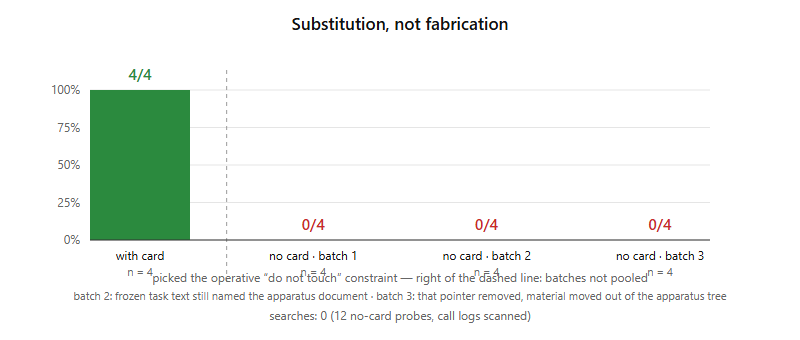
\includegraphics[keepaspectratio]{fig4-behavioral.png}}

\textbf{Figure 4.} Behavioral probes: 4 / 4 windows retrieved the
operative constraint when the material arrived with a retrieval card;
without one, three independent batches returned 0 / 4 each (batches not
pooled --- §5).

Understanding is not doing. We therefore ran a second, behavioral
measurement: probes receive the same frozen material as above, delivered
either as \textbf{material without a retrieval card} or \textbf{material
with a card} carrying one line that states the operative constraint and
its reason. Each probe must produce a \texttt{next} pointer file plus a
reason. Two columns are scored: which ``do not touch'' constraint it
selected, and whether it searched.

{\def\LTcaptype{none} % do not increment counter
\begin{longtable}[]{@{}
  >{\raggedright\arraybackslash}p{(\linewidth - 6\tabcolsep) * \real{0.2500}}
  >{\raggedright\arraybackslash}p{(\linewidth - 6\tabcolsep) * \real{0.2500}}
  >{\raggedright\arraybackslash}p{(\linewidth - 6\tabcolsep) * \real{0.2500}}
  >{\raggedright\arraybackslash}p{(\linewidth - 6\tabcolsep) * \real{0.2500}}@{}}
\toprule\noalign{}
\begin{minipage}[b]{\linewidth}\raggedright
Arm
\end{minipage} & \begin{minipage}[b]{\linewidth}\raggedright
n
\end{minipage} & \begin{minipage}[b]{\linewidth}\raggedright
selected the operative constraint
\end{minipage} & \begin{minipage}[b]{\linewidth}\raggedright
searches
\end{minipage} \\
\midrule\noalign{}
\endhead
\bottomrule\noalign{}
\endlastfoot
with card & 4 & \textbf{4/4} & 0 \\
without card --- batch 1 & 4 & \textbf{0/4} & 0 \\
without card --- batch 2 \emph{(frozen task text still named the
apparatus document that records the answer)} & 4 & \textbf{0/4} & --- \\
without card --- batch 3 \emph{(that pointer removed; material moved out
of the apparatus tree)} & 4 & \textbf{0/4} & 0 \\
\end{longtable}
}

The failures are informative. In batch 1, three probes selected a
standing constraint that \textbf{does} appear verbatim in the material's
\texttt{\#\#\ Boundaries} --- one that is real, but not the one
governing this task --- and one selected a different file that also
appears in the material. Counting occurrences in the material explains
\textbf{that} batch: the operative constraint appears \textbf{0} times
without the card and 3 times with it; the substituted constraint appears
3 times in both. \textbf{It does not explain batch 3}: same material,
pointer removed, and the four probes took the material's standing
constraint twice, their own material path once, and the repository root
once. Batches 2 and 3 are therefore \textbf{not pooled} with batch 1 ---
the three windows could see different things --- and the mechanism claim
is scoped accordingly: \textbf{the zero is the invariant; the substitute
is not}.

This is \textbf{substitution}: not invention, but the capture of
whatever constraint is nearest to hand --- and, crucially,
\textbf{without any marker of uncertainty}. The probes did not say ``I
am guessing''; they filled the slot. For safety-relevant behavior a
confidently substituted constraint is worse than an acknowledged
unknown, because nothing downstream flags it: the file gets written, the
slot is filled, and the error is invisible until something acts on it.

We observed the same shape in three different material families earlier
in the line: a material with no correct item present produced
\emph{substitution} (4/4 probes picked the nearest real constraint); a
material that contained identifiers but no constraints produced an
honest ``cannot find a basis'' (2/2); a material containing the real
constraint plus a competing one produced \emph{selection} (3/8 and 6/8
depending on order). The failure shape is a property of the material,
not a single disease.

Across the first eight behavioral probes the number of searches was
\textbf{0} (7--13 tool calls each, all within the supplied material plus
writing their own output file); the four probes of batch 3 were also
\textbf{0/4}. This is the first number we can attach to the design goal
``continuity without searching.''

\subsection{Alternative explanations we could not rule
out}\label{alternative-explanations-we-could-not-rule-out-3}

\begin{itemize}
\tightlist
\item
  \textbf{Task difficulty.} A harder task might have produced searching,
  or an explicit ``I don't know''. Our task was small on purpose: it
  isolates \emph{which} constraint is carried, not whether the window
  can do the work.
\item
  \textbf{Zero-history probes are not working windows.} A real window
  has its own context, its own recent actions, and its own stake in the
  outcome. Nothing here shows how a working window behaves after a real
  compaction; the one observation we have from a working window (n=1,
  the authors' own) is that it answered from context without reading
  files, and that its retrieved pointer was \emph{stale} --- consistent
  with §3 but not a distribution.
\item
  \textbf{The card may be doing something else.} We assume the card
  works because it contains the constraint verbatim. An equally
  consistent account is that it works because it is \emph{short}: a
  one-line carrier is easy to read. We did not run a short-but-wrong
  card.
\end{itemize}

\begin{quote}
\textbf{Threat note.} ``Compaction erases constraints'' and ``plans are
evicted early'' are established. What we have not seen measured is the
\textbf{shape of the failure after erasure} --- a near neighbour
substituted with full confidence --- nor its behavioral consequence in a
real deployment.
\end{quote}

\section{6. Related work}\label{related-work}

Nine recent works bear directly on this one. We list what each
contributes, and what remains for a deployment study.

\begin{itemize}
\tightlist
\item
  \textbf{Compaction Cliff} (arXiv:2608.22752) --- measures safety-rule
  recall decaying 53\% → 10\% over five rounds on a production-style
  prompt, and proposes type-conditioned retention. Establishes that
  \emph{content} decays and that retention policies should not be
  type-blind. We measure the same phenomenon on real sessions, in two
  rulers, and add the failure classes that occur \emph{below} the output
  floor.
\item
  \textbf{Governance Decay} (arXiv:2606.22528) --- shows compaction
  silently erasing governance constraints, quantified by
  \textbf{ConstraintRot, a benchmark of self-contained long-horizon
  agent scenarios with deterministic violation grading} (plus a
  real-harness validation across production agent-framework context
  managers, §8), with \textbf{Constraint Pinning} as a remedy --- a
  \textbf{training-free mitigation that quarantines the constraint from
  lossy compaction, re-injects it, and integrity-checks it across
  turns}. Our contribution is what happens in the \emph{absence} of such
  a policy, on real material: substitution without a marker.
\item
  \textbf{Lost in Compaction / COMPINT} (arXiv:2608.11242) --- names
  \textbf{Session Constraints} (user instructions meant to bind the rest
  of a session) and measures their loss with a purpose-built suite
  across multi-turn chat, agentic trajectories and long-horizon
  research: current compactors retain \textbf{17\% of injected
  constraints on average}, and \textbf{most perform worse than not
  compacting at all}. Retention varies with compactor, prompt, context
  length, constraint phrasing and injection location, so the loss is
  \textbf{systematic rather than a bad setting} --- and they answer it
  on the extractor side (an SC-aware extractor). This is the closest
  prior statement of the §4 phenomenon, and it sharpens what is ours:
  they \textbf{inject} constraints into constructed scenarios and score
  \textbf{retention}; we measure \textbf{real deployment logs} under
  \textbf{two rulers} (13\% verbatim vs 91 / 77 / 53\% semantic, §4) and
  add what happens \textbf{after} erasure --- a near neighbour
  substituted with full confidence and no marker (§5) --- which a
  retention rate cannot show. Their headline (``most compactors do worse
  than no compaction'') is also the second independent argument against
  reading our positive state results as a fix.
\item
  \textbf{Plans Don't Persist} (arXiv:2606.22953) --- one-step
  plan-signal decay (4.1×) and a compression stress test showing 56.7\%
  → 22.0\% success after naive eviction, with no recovery from plan
  protection (20.7\%, p = 0.89) or probe-gated re-surfacing (24.7\%, p =
  0.67), despite 6.1 re-insertions. This is the strongest argument
  against reading our positive state results as a fix.
\item
  \textbf{Beyond Compaction / CWL} (arXiv:2606.11213) --- typed,
  dependency-linked episodes with deterministic, \textbf{LLM-free}
  eviction. Establishes \textbf{deterministic, LLM-free eviction over
  agent-declared typed episodes} as a system design; we observe that in
  a deployment, deterministic artifacts exist but have \textbf{no
  automatic reader} (they are read 0 times unless something triggers a
  read).
\item
  \textbf{Parallel Context Compaction} (arXiv:2605.23296) ---
  summarization \textbf{output volume is essentially input- and
  prompt-invariant} (input grows 48×, output \textasciitilde3×; the
  model self-bounds its output) and \textbf{synchronous compaction
  dominates wall time at low thresholds} (up to 62\% of end-to-end
  execution). Establishes the output floor we cite in §2.
\item
  \textbf{Rate--Distortion survey} (arXiv:2607.08032) --- unifies
  compression approaches \textbf{under one rate--distortion objective
  and promotes reversibility and query-conditioning}. Its
  \textbf{(P-fid) fidelity profile} axis is adjacent to what our two
  rulers separate: preserving \emph{wording} and preserving
  \emph{meaning} are different targets --- and its own (P-rev)
  reversibility axis is about re-derivation on demand, not about
  wording.
\item
  \textbf{Aging / AgingBench} (arXiv:2605.26302) --- names
  deployment-time agent aging and measures it with a synthetic generator
  plus longitudinal statistics (half-life, decay slope), noting that
  production telemetry is an open frontier. This paper is a data point
  on that frontier --- and a demonstration that one of its rulers cannot
  be transplanted to logs that lack per-session capability scores.
\item
  \textbf{SHARP} (arXiv:2605.06822; policy evolution under a validation
  gate) --- in a different domain, names the failure we measure in §5:
  unbounded text rewrites can \textbf{silently overwrite previously
  correct behavior} (\emph{policy degeneration}) in ways a validation
  gate \emph{cannot fully catch}. Its controlled ablation is the
  cleanest available statement that structure in the \textbf{mutation
  operator} --- not model or budget --- decides the outcome: same
  validation gate and same evolution budget, only rule-editing replaced
  by free-form rewriting, and \textbf{on GPT-4o-mini} performance falls
  \textbf{below the no-adaptation baseline} (Sharpe +2.45 → -0.84; total
  return +33.2\% → -12.1\%, against \textbf{+7.3\% static}). On the
  second backbone the same ablation lands at \textbf{+6.0\%} versus a
  static baseline of \textbf{-6.4\%} --- above static, still well below
  full adaptation (+22.9\%) --- so the \emph{size} of the degradation is
  backbone-dependent while the free-form variant trails full adaptation
  on both. The same paper reports the shape we measure: the free-form
  variant ``gradually shifts \ldots{} into flowing prose whose
  thresholds drift without any traceable link to specific error days''.
  We measure the same family on real deployment logs (substitution
  without a marker, §5) rather than through a downstream reward.
\end{itemize}

\textbf{One axis we probed three times, because it is the axis we would
most like to have: \emph{which harness}.} Across the \textbf{eight works
in that scan} (the ninth entry above was added after that scan --- its
own axes are compactor, prompt, context length, constraint phrasing and
injection location, again \textbf{not} implementation), the comparison
axes are model (5), task (5), run (3), session (3), benchmark / domain /
layer (2 each), backbone / scenario / seed / strategy (1 each) ---
\emph{implementation} is none of them (device, spans and controls in
\texttt{report/prior-art-cross-impl.md}). The two nearest runs vary the
container while holding the compactor fixed: Governance Decay §8 injects
the \emph{same} LLM-written compacted summary into LangGraph, LangMem,
AutoGen's \texttt{BufferedChatCompletionContext} and an OpenAI Agents
SDK Runner, and labels its SDK case ``an SDK integration check rather
than a claim about SDK-native compaction''; AgingBench does run ReAct,
OpenHands and Claude Code --- including production CLI agents with
recompaction events --- but scores the \textbf{aging curve}, with the
memory policy and compaction prompt supplied by its runner (App. F.3).
The rate--distortion survey's own §13.2 names the same gap we address:
no suite checks ``whether a scheme knows what it dropped, whether it can
get it back, and whether its confidence reflects what it kept''. So our
claim is a first measurement \textbf{on an unoccupied axis}, not a
cross-implementation comparison: the harness that produced our results
is one. What we can say about the devices is narrower and stronger than
``portable'': the two things a device must know about a corpus ---
\emph{how logs are stored} and \emph{what the events are called} --- are
isolated in one editable table (\texttt{tools/foreign-log-adapter.mjs}),
and the device now runs on \textbf{two harnesses' native logs}, verified
against independent counts on both (see §9 and
\texttt{report/cross-harness.md}). \textbf{Our own measuring side has
since crossed one implementation boundary in the other direction}:
pointed at \textbf{198 native transcripts from a different harness}, the
adapter paired \textbf{29 of 29} generations at id level and the
independent counts agreed (§9) --- the axis is empty in the literature
while being \emph{traversable} by the apparatus.

\textbf{What a head-to-head would require.} We deliberately do not place
our numbers beside anyone else's, and the reason is not modesty: a
numeric comparison is only meaningful when three things match --- the
same material, the same \textbf{frozen} criterion, and the same round
\emph{k}. Two of our results are portable in that sense: the verbatim
curve is defined by normalized 5-gram containment and the semantic curve
by a written three-state rule, both fixed before use, so a reader can
re-run those criteria on their own summaries and obtain a comparable
number --- that is the comparison we would rather invite. The third
result is \textbf{not} portable: it measures whether a retrieval card
changes what a window does, which is a property of one deployment's
apparatus rather than of summaries. The one cross-material reading we do
report (§9) compares \emph{material and compaction regime}, not
implementations. And where a prior work states a same-shaped claim on a
different ruler --- Compaction Cliff's 53\% → 10\% recall of safety
rules --- we cite it as a claim (threat note under §1) and we do not
subtract our curve from theirs.

\section{7. What we do not claim}\label{what-we-do-not-claim}

{\def\LTcaptype{none} % do not increment counter
\begin{longtable}[]{@{}
  >{\raggedright\arraybackslash}p{(\linewidth - 2\tabcolsep) * \real{0.5000}}
  >{\raggedright\arraybackslash}p{(\linewidth - 2\tabcolsep) * \real{0.5000}}@{}}
\toprule\noalign{}
\begin{minipage}[b]{\linewidth}\raggedright
Claim we would like to make
\end{minipage} & \begin{minipage}[b]{\linewidth}\raggedright
Already established by
\end{minipage} \\
\midrule\noalign{}
\endhead
\bottomrule\noalign{}
\endlastfoot
Compaction erases constraints and rules & Compaction Cliff; Governance
Decay (with a benchmark) \\
Plans and pointers are the first to decay & Plans Don't Persist \\
Reversible memory beats irreversible memory & Rate--Distortion survey \\
Retain by pinning (Governance Decay) / by agent-declared structure (CWL)
rather than by detecting stability & Governance Decay (pinning);
Compaction Cliff (per-type); Beyond Compaction (agent-declared
episodes) \\
Models largely ignore compaction length instructions & Parallel
Compaction \\
Deterministic, LLM-free eviction over agent-declared episodes can
replace LLM rewriting & Beyond Compaction (CWL) \\
Unbounded free-text rewriting silently degrades previously-correct
behavior, and a validation gate cannot fully catch it & SHARP
(arXiv:2605.06822, \emph{policy degeneration}; controlled A2
ablation) \\
\end{longtable}
}

We also do \textbf{not} claim that a retrieval card fixes behavior. The
strongest available evidence points the other way (§6).

\section{8. Limitations}\label{limitations}

\begin{enumerate}
\def\labelenumi{\arabic{enumi}.}
\tightlist
\item
  \textbf{One deployment, one person.} 48 sessions from a single machine
  are a case study, not a distribution. Treat every rate here as an
  existence proof plus a first measurement.
\item
  \textbf{Self-judged.} All thresholds were fixed by us before use; the
  semantic column was produced by zero-history judges instantiated by
  the same system. \textbf{Two machine passes} now exist (ten
  zero-history judges each, one pack per judge, all 56 cells):
  de-duplicated agreement \textbf{52.2\% / \ensuremath{\kappa} = 0.226},
  and \textbf{54.3\% / \ensuremath{\kappa} = 0.261} after we
  disambiguated our own three-state rule --- the rule fix moved it by
  \textasciitilde2 points, so the residual is \textbf{judgment
  variance}, not the wording. On the two states the survival curve uses,
  the two passes give \textbf{87.5\% / \ensuremath{\kappa} = 0.470} and
  \textbf{83.9\% / \ensuremath{\kappa} = 0.319} (per cell; de-duplicated
  87.0\% / \ensuremath{\kappa} = 0.502 and 82.6\% / \ensuremath{\kappa}
  = 0.336): quote the range.

  \begin{itemize}
  \tightlist
  \item
    The two passes agree with \textbf{each other} on 75.0\% of cells
    while each agrees with the key at 55--57\%; a \textbf{third pass},
    on the same material but judged one cell at a time, shows that two
    windows agreeing is \textbf{not} consensus --- with three windows
    the key stands alone on \textbf{3 of 56} cells on the two-state
    boundary while the windows disagree among themselves on \textbf{6},
    so we no longer claim the key is the outlier. The third pass is
    nearest to the key (92.9\% two-state) but \textbf{not significantly}
    so (McNemar exact, p = 0.063--0.38).
  \item
    A \textbf{cross-model pass} (a different vendor's model, same packs
    and rule) agrees with the key at 64.3\% three-state / 89.3\%
    two-state and is not an outlier either; with four judges the key
    stands alone on \textbf{2 of 56} boundary cells --- but judge counts
    are not comparable to one another (more judges make consensus
    harder), so we read that as ``no systematic outlier at any count'',
    not as a trend. Both are \emph{repeat-run stability} figures, not
    human agreement, and 56 cells support no significance claim between
    runs.
  \item
    \textbf{A human pass now exists}: one author, blind to the key,
    labelled all 56 cells under the original three-state rule ---
    de-duplicated agreement \textbf{56.5\% / \ensuremath{\kappa} =
    0.291}, i.e.~\textbf{at or above both machine passes} (our earlier
    prediction that a human-versus-model figure must be lower is
    \textbf{falsified}, and is recorded as a retraction), and on the two
    states the curve uses \textbf{89.1\% / \ensuremath{\kappa} = 0.556},
    the closest of the three raters to the key, with her disagreements
    on the same \texttt{verbatim} \ensuremath{\leftrightarrow}
    \texttt{reworded} edge (\textbf{19 of 24}). What is still missing is
    not a human but a \textbf{non-author} human: the inter-annotator
    number remains n = 1, and the key is written by the agent half of
    the same pair.
  \item
    \textbf{Three further readers, one from each of three different
    model families} (blind to the key, one pack at a time in order, one
    session each) were added after this list was first written; they are
    reported as \textbf{their own arm} in §4 and are \textbf{not} folded
    into the judge counts above, because those counts depend on which
    judges are included. Their disagreements with the key sit
    \textbf{entirely off the two-state boundary} --- \textbf{0} cells at
    \texttt{verbatim} \ensuremath{\leftrightarrow} \texttt{gone} against
    \textbf{14 / 16 / 17} at \texttt{verbatim}
    \ensuremath{\leftrightarrow} \texttt{reworded} --- which is the same
    seam every other pass falls on.
  \end{itemize}
\item
  \textbf{Small n --- intervals where counts exist, reader spread
  everywhere else.} Survival curves: 10 sessions / 56 items, with
  \textbf{Wilson 95\% intervals} at k = 1 (7/56 → 6--24\%, 51/56 →
  81--96\%); at k = 2 and k = 4 the dominant uncertainty is
  \textbf{reader spread}, which we report per point rather than as an
  interval. Behavioral: 4 probes per arm in the first batch, and 12
  no-card probes across three batches that are \textbf{not pooled}
  (their windows could see different things) --- at n = 4 per batch we
  quote no interval at all.
\item
  \textbf{Transplanted rulers.} Where a published ruler could not be
  transplanted (AgingBench's half-life), we say so rather than
  substituting a different quantity silently.
\item
  \textbf{No success metric.} We did not measure whether tasks succeeded
  more often; that requires a task suite we do not have.
\item
  \textbf{Failure counts are attempts.} See §2.
\item
  \textbf{The probes were not fully blind to the apparatus --- and we
  can say exactly which channel stayed open.} Two channels could hand a
  window the answer: the frozen task text of one batch named the
  apparatus document that records the probe's answer, and every later
  batch carried the \textbf{author's own working notes} --- which
  mention the discriminator --- in its injected context. We scanned each
  batch's session log for both channels rather than assuming blindness:
  batch 1 shows no trace of either; batch 2 shows traces of the document
  channel; batch 3 (materials and prompt moved out of the apparatus
  tree) closed the document channel at \textbf{0 traces}, while the note
  channel remained and is \textbf{quantified}: three string families
  unique to our own notes appear in all four probes' injected context at
  identical counts (4, 13 and 6), which is what tells us they come from
  injection and not from the probes' own writing. We then edited the
  note that carried the discriminators out of the line's own injected
  map (re-count for those families in that file: 0), but the same
  wording also lives in the author's durable memory, and
  \textbf{injection is not configurable per run from inside the
  deployment} --- so a fully blind condition needs a \emph{different}
  deployment or agent, not another batch, and we report that as the
  residual rather than as an achieved control. The zero itself
  replicated under all three conditions --- normal prompt, non-blind
  prompt, and prompt-with-pointer-removed --- which is why we call it
  the invariant, and the apparatus defect found this way (a frozen task
  text that still pointed at the apparatus document) is recorded in the
  line's own notes.
\end{enumerate}

\section{9. Reproducibility}\label{reproducibility}

Every number above is produced by one of six devices in \texttt{tools/},
all of which run on ordinary session logs and print the criterion they
apply:

{\def\LTcaptype{none} % do not increment counter
\begin{longtable}[]{@{}
  >{\raggedright\arraybackslash}p{(\linewidth - 4\tabcolsep) * \real{0.5000}}
  >{\raggedright\arraybackslash}p{(\linewidth - 4\tabcolsep) * \real{0.3100}}
  >{\raggedright\arraybackslash}p{(\linewidth - 4\tabcolsep) * \real{0.1900}}@{}}
\toprule\noalign{}
\begin{minipage}[b]{\linewidth}\raggedright
Device
\end{minipage} & \begin{minipage}[b]{\linewidth}\raggedright
Measures
\end{minipage} & \begin{minipage}[b]{\linewidth}\raggedright
Input
\end{minipage} \\
\midrule\noalign{}
\endhead
\bottomrule\noalign{}
\endlastfoot
\texttt{compaction-census.mjs} & success/failure per session, shadowed
tokens, receipts & session logs \\
\texttt{constraint-survival.mjs} & verbatim survival curve & census
dump \\
\texttt{constraint-survival-pack.mjs} & builds self-contained judgment
packs & census dump \\
\texttt{semantic-survival-tally.mjs} & aggregates three-state judgments
& judge answers \\
\texttt{probe-toolcalls.mjs} & tool calls and search count from a
probe's own log & session log \\
\texttt{scan-prior-art-axes.mjs} & which comparison axes a body of prior
work uses, with positive/negative controls (§6) & a directory of arXiv
HTML \\
\end{longtable}
}

All six were executed inside the published tree before release and
reproduce the numbers in this report (\texttt{README.md} records the
check). Thresholds live in the device headers, not in this text. The
protocol for the probe runs --- material/question/key discipline, the
three scoring columns, the search-counting rule with its two traps, and
the registration rules --- is in \texttt{tools/PROTOCOL.md}. The §6 axis
tally, its verbatim spans and its controls are in
\texttt{report/prior-art-cross-impl.md}.

\textbf{A portability test, and what it caught.}
\texttt{tools/foreign-log-adapter.mjs} isolates the two things a
log-reading device must know about a corpus --- \emph{container/layout}
(here: multi-frame zstd, gzip JSONL, plain JSONL) and \emph{event
vocabulary} (a rename table plus field aliases) --- into tables, so
pointing a device at another harness means editing a table rather than
the logic. \texttt{tools/make-foreign-fixture.mjs} then generates a
\textbf{synthetic log in a deliberately foreign shape} (plain/gzip
JSONL, events named \texttt{ctx.compact} / \texttt{ctx.compacted} /
\texttt{ctx.compact\_receipt}, fields named \texttt{tokensShadowed} /
\texttt{seqs} / \texttt{cid}) and states the numbers the census must
print. Running it end to end found a defect that had nothing to do with
the second harness:

\begin{quote}
The census matched each \texttt{compaction/start} to its summary by
\textbf{\texttt{seq} equality}. On this corpus that assumption never
holds (\texttt{start} seq 129,373 / \texttt{summary} seq 129,374), so
the section headed \emph{``triggered a start but produced no summary''}
was listing \textbf{every} start --- all 36 in the deepest session, of
which 30 had in fact produced summaries. The correct key is
\texttt{compactionId}, which all four event kinds carry. After the fix
the same session reports \textbf{6} unpaired starts (36 - 30) and the
one genuinely unclosed start is unchanged.
\end{quote}

Two things generalize. First, \textbf{a detector that always fires looks
like a finding}: this section had been printed, read, and quoted in our
own notes as a real property of the corpus. Second, the cheap way to
find that class of error is to \textbf{run the device on an input whose
expected output you know}, which is exactly what a synthetic fixture
gives you --- the same discipline as the empty-input guard, applied to
the \emph{shape} of the input rather than its presence.

\textbf{And then a real second harness appeared.} After the synthetic
fixture, the same adapter was pointed at a genuinely foreign corpus that
happened to exist on the same machine: \textbf{198 native transcripts
from a different agent harness} (plain JSONL, so the container seam
matched immediately). Compaction is not named as an event there; it is
marked by a boolean field and a subtype. Adding two predicate rules to
the adapter table ---
\texttt{system}+\texttt{subtype:\textquotesingle{}compact\_boundary\textquotesingle{}}
→ the accounting record, \texttt{user}+\texttt{isCompactSummary:true} →
the summary record --- was enough for the census to run on it. On the
largest transcript (\textbf{11,241 records, 29.4 MB}) the census reports
\textbf{29 compactions}, matching an \textbf{independent count of the 29
boundary records}, and a shadowed-token total of \textbf{4,905,460},
matching an independent sum of the same field. Pairing between the two
record kinds was established by an \textbf{id, not by adjacency}
(\texttt{summary.parentUuid\ ==\ boundary.uuid}, holding \textbf{29/29})
--- deliberately, because assuming an identity from position is the
defect reported above.

Three limits we state rather than bury: (i) the token field we map to
``shadowed'' is the \emph{pre-compaction context size}, so it is an
\textbf{upper bound}, not the same quantity our dsh numbers report; (ii)
that corpus records \textbf{no failures}, so \texttt{0\ failures} there
means \emph{not visible}, not \emph{none happened}; (iii) the \textbf{§4
ruler did not transfer} --- see below. Our claim therefore remains what
§6 says: a first measurement on an unoccupied axis, with a device
demonstrated on two harnesses and real results from one. The foreign
transcripts stay out of the artifact entirely: no upstream text is
quoted, and the readings are counts, field names and rates.

\textbf{What did not transfer, and what did instead.} Our constraint
ruler keys on a \textbf{named section} of the summary. The second
harness's summaries contain \textbf{no \texttt{\#\#} heading at all} ---
0 of 29 generations --- so that ruler extracts nothing there, and we
report \emph{zero items found} rather than a percentage (an empty
extraction is not a measurement of zero). A \textbf{structure-free
variant} of the same survival question keeps the identical containment
criterion and changes exactly one thing --- items are bullet lines
\emph{anywhere} in the summary --- and runs on both harnesses. Its
reading is not harness-shaped: the two long sessions, one per harness,
keep \textbf{4\%} and \textbf{5\%} of their first generation's items
verbatim after one round, while a dsh \textbf{burst-regime} session
keeps \textbf{71\%}. In this sample the variable that separates them is
the session's compaction regime, not the harness. Limits: the item class
is bullet-level items, \textbf{not} constraints; one session per
harness; regimes unmatched; k = 0 is 100\% by construction and is used
as the device's own fixpoint check. Details and the full 12-session
table: \texttt{report/cross-harness.md}.

\textbf{The invariants the census never checked.} The same fixture
carries a second corpus that is \emph{deliberately broken}, plus a
look-alike negative control, and
\texttt{tools/audit-census-invariants.mjs} turns the census's implicit
counting assumptions into four stated invariants: (i) one summary per
\texttt{compactionId} (otherwise a retry is counted as a second
success), (ii) every summary carries a shadowed-token count (otherwise
the shadowed total is silently low), (iii) checkpoint \texttt{seq}s are
unique (otherwise the carried-over-text numerator double-counts), (iv)
every \texttt{start} carries the pairing key (the ERR-047 failure,
inverted). On this corpus all four \textbf{hold} --- 660 log files, 258
summaries, 303 starts, 258 checkpoints (\textbf{snapshot 2026-09-22
16:44}) --- and on the decoy corpus the audit goes red on exactly the
three invariants it should, with the offending records named.
\textbf{These counts are not the headline counts, and the difference is
the point}: they come from a \emph{later} run of the same store, which
keeps growing (the headline snapshot at 2026-09-19 00:3x counted 203
compactions, this run counts 258 summaries); every corpus-level number
in this paper is paired with the moment it was read, and this is what
that discipline looks like when the corpus is alive. The look-alike
control is the one that tests \emph{membership}: a message from a
different plugin whose text is shaped like a summary is \textbf{not}
counted as a checkpoint (criterion is the \texttt{source.plugin} field,
not the content's shape).

\textbf{Three defects came out of our own tooling, and all three answer
a different question without erroring}: the census read its workspace
filter from the \textbf{fourth} positional slot, so the intuitive
\texttt{list\ \textless{}scope\textgreater{}} printed the whole library
--- formatted exactly like a scoped answer (it now takes
\texttt{-\/-scope} and warns when an argument is ignored); a device
pointed at the wrong input directory printed an \textbf{empty table and
exited 0}; and the front page had no copy-pasteable command, with paths
that only worked on our machine. What found them was a cold read of this
artifact as a stranger would read it, following the quickstart
literally; their generalised forms are items (iv)--(vi) of the checklist
below. We record the family because it is the failure mode of exactly
this kind of work: the numbers are reproducible \emph{in the authors'
environment} while the artifact silently fails elsewhere. \textbf{Data.}
We publish code and \textbf{aggregate, anonymized} columns
(\texttt{data/sessions.md}, one row per session). We do \textbf{not}
publish session transcripts or summary texts: they contain one person's
private work and personal context, and our policy
(\texttt{DATA-POLICY.md}) treats that as non-publishable regardless of
research value.

\textbf{A checklist for anyone repeating this.} (i) Fix a snapshot and
print it beside every corpus number. (ii) Measure the noise floor before
interpreting an arm difference. (iii) Pick the discriminating column
before the run (\texttt{{[}guess{]}} beats totals in our experience) and
keep the frozen key untouched when it turns out too narrow --- add a
second key. (iv) Verify tool-argument key names against a dumped raw
event; they are harness-version dependent. (v) When a device is copied
into a publishable tree, de-identify it and re-run it there before
claiming it works. (vi) \textbf{Give every device an input whose answer
you already know.} We found three defects this way in one night, and not
one of them was about the data: an empty input that printed a plausible
table and exited 0; a pair of event kinds matched by position instead of
by id, so a section headed ``triggered but produced no summary'' listed
\emph{every} attempt; and a filter read from the wrong argument slot, so
a scoped query silently answered the whole-corpus question. (vii)
\textbf{Also give it an input you know is broken.} A detector whose
predicate is always true prints a list that looks like a finding; a
corpus that deliberately violates each invariant is the cheapest way to
prove your checker is not permanently green. (viii) \textbf{Assert a
fixpoint.} Our first version of one device produced \textasciitilde0\%
on both harnesses --- plausible as a result, and wrong, because a
callback signature bug made every item after the first incomparable. Its
saving grace was a cell that must be 100\% by construction (a baseline
compared against its own generation), now an assertion that fails
loudly. Three cheap questions, each one asked of the device rather than
of the world: \emph{empty? known-good? known-bad? fixpoint?}

\section{References}\label{references}

Metadata (title, author list, submission date) was checked against the
arXiv API on 2026-09-20; each id matches the inline citations in §6.

\begin{enumerate}
\def\labelenumi{\arabic{enumi}.}
\tightlist
\item
  X. Chen, W. Zhu, S. Zheng, K. Rasul, Y. Deng, H. Li. \emph{SHARP: A
  Self-Evolving Human-Auditable Rubric Policy for Financial Trading
  Agents.} arXiv:2605.06822 (2026).
\item
  M. Cim, B. Topcu, C. Das, M. T. Kandemir. \emph{Parallel Context
  Compaction for Long-Horizon LLM Agent Serving.} arXiv:2605.23296
  (2026).
\item
  J. Zhu, Y. Ro, J. Robertson, K. Wang, J. Li, H. Vikalo, A. Akella, Z.
  Wang. \emph{Your Agents Are Aging Too: Agent Lifespan Engineering for
  Deployed Systems.} arXiv:2605.26302 (2026).
\item
  A. Semenov, S. Dorofeev. \emph{Beyond Compaction: Structured Context
  Eviction for Long-Horizon Agents.} arXiv:2606.11213 (2026).
\item
  S. Chen. \emph{Governance Decay: How Context Compaction Silently
  Erases Safety Constraints in Long-Horizon LLM Agents.}
  arXiv:2606.22528 (2026).
\item
  A. Mehta, A. Datta. \emph{Plans Don't Persist: Why Context Management
  Is Load Bearing for LLM Agents.} arXiv:2606.22953 (2026).
\item
  A. G. Colaco, N. Lahjouji. \emph{What to Keep, What to Forget: A
  Rate--Distortion View of Memory Compaction in LLMs and Agents.}
  arXiv:2607.08032 (2026).
\item
  Z. Wang, Y. Zhang, D. Lee, Y. Yang. \emph{Lost in Compaction:
  Evaluating Side-Constraint Loss under Context Compaction.}
  arXiv:2608.11242 (2026).
\item
  S. Zerhoudi, J. Mitrovic, M. Granitzer. \emph{The Compaction Cliff in
  Long-Running AI Agent Memory.} arXiv:2608.22752 (2026).
\end{enumerate}

\textbf{Policy document.} arXiv. \emph{Policy for authors' use of
generative AI language tools} (moderation policy).
\texttt{https://info.arxiv.org/help/moderation} --- accessed 2026-09-20.

\section{Appendix A --- per-session aggregate
table}\label{appendix-a-per-session-aggregate-table}

See \texttt{data/sessions.md} (48 rows; anonymized identifiers; columns:
successful compactions, failed attempts, shadowed tokens, log size).
Per-session failure \emph{classification} is not available: it would
require re-decoding every log, and we state the aggregate-only result
rather than implying precision.

\section{Appendix B --- judgment protocol (semantic
ruler)}\label{appendix-b-judgment-protocol-semantic-ruler}

Each pack contains: (a) the numbered constraint list from the first
generation; (b) the full text of the summary after k rounds; (c) the
three-state rule with an explicit fallback (``if not found, write
\texttt{gone}''). Judges are zero-history: they read only their own
pack, are forbidden from searching anything else, and must quote a basis
for each verdict. Aggregated by \texttt{semantic-survival-tally.mjs}.
The machine second pass reused these packs unchanged. \textbf{The human
pass has now been run on the same packs} --- one author, no access to
the key, all 56 cells --- under the \textbf{original} three-state rule
this pack carries, not the disambiguated rule written afterwards (§8
reports the second pass under that one). Its agreement figures are in §4
and §8; the filled table and its scoring output stay in the annotation
workspace and are not part of this tree.

\end{document}
